\documentclass[landscape, 8pt]{extarticle}
\usepackage{geometry}
% \usepackage{showframe}

\geometry{
    a4paper, 
    margin=0.2in
}

\usepackage{graphicx} % Required for inserting images
\usepackage{amsmath}
\usepackage{amsfonts}
\usepackage{preamble}
\usepackage{multicol}
\usepackage{lipsum}
\usepackage[framemethod=TikZ]{mdframed}
\usepackage{thmboxes}
\usepackage{float}
% \usepackage{setspace}
\usepackage[nodisplayskipstretch]{setspace}

% \setlength{\parskip}{0pt}

\DeclareMathOperator{\Ima}{im}
\DeclareMathOperator{\Fix}{Fix}
\DeclareMathOperator{\Orb}{Orb}
\DeclareMathOperator{\Stab}{Stab}
\DeclareMathOperator{\send}{send}

\begin{document}

\setlength{\abovedisplayskip}{4pt}
\setlength{\belowdisplayskip}{4pt}
\setlength{\abovedisplayshortskip}{4pt}
\setlength{\belowdisplayshortskip}{4pt}

\begin{multicols}{3}
\raggedcolumns
\section{\huge Algebra}
\subsection*{Functions and Symmetries}

\begin{dfn}[Functions]{def:functions}{0.1.1}
A function $f:X\to Y$ is called
\renewcommand\labelitemi{\tiny$\bullet$}
\begin{itemize}
    \setlength\itemsep{0em}
    \item \textbf{injective} if $f(x_{1}) = f(x_{2}) \implies x_{1} = x_{{2}}$
    \item \textbf{surjective} if for every $y\in Y,\, \exists x\in X$ s.t. $f(x) = y$
    \item \textbf{bijective} if it is both injective and surjective
\end{itemize}
% \begin{figure}[H]
%     \centering
%     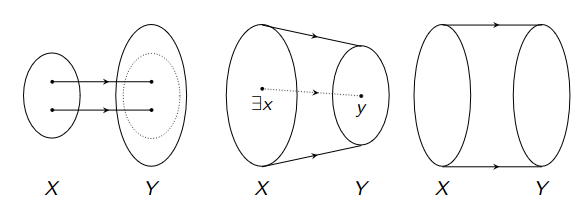
\includegraphics[width=\linewidth]{images/functions.png}
% \end{figure}
\end{dfn}
\vspace{-5pt}

\begin{dfn}[Graph Isomorphisms]{def:graph-iso}{1.1.3}
    An \textbf{isomorphism} between two graphs is a \textit{bijection} between them that preserves all edges. More precisely, if $\Gamma_{1}$ and $\Gamma_{2}$ are graphs, with sets of vertices $V_{1}$ and $V_{2}$ respectively, then an isomorphism from $\Gamma_{1}$ and $\Gamma_{2}$ is a bijection
    \[f : V_{1}\to V_{2}\]
    such that $f(v_{1})$ and $f(v_{2})$ are joined by an edge if and only if $v_{1}$ and $v_{2}$ are also joined by an edge.
    We say that $\Gamma_{1}$ and $\Gamma_{2}$ are \textit{isomorphic} if there exists an isomorphism $f:\Gamma_{1}\to\Gamma_{2}$
\end{dfn}
\vspace{-5pt}

\begin{dfn}[Symmetry]{def:symmetry}{1.1.9}
    A \textbf{symmetry} of a graph is an \textit{isomorphism} from the graph to itself, i.e. if the set of vertices is V, then the symmetry is a bijection $f:V\to V$ that preserves edges. That is, a symmetry is a bijection $f:V\to V$ such that $f(v_{1})$ and $f(v_{2})$ are joined by an edge if and only if $v_{1}$ and $v_{2}$ are joined by an edge.
\end{dfn}
\vspace{-5pt}

% -------------------------------------

\subsection*{Groups}

\begin{dfn}[Groups]{def:group-def}{1.2.3}
    For an operation $\ast$, We say a non-empty set G is a \textbf{group} under $\ast$ if the following four axioms hold:
    \renewcommand\labelitemi{\tiny$\bullet$}
    \begin{itemize}
        \setlength\itemsep{0em}
        \item \textbf{G1 - Closure:} $\ast$ is a binary operation on G, that is $a\ast b \in G$ for all $a,b\in G$.
        \item \textbf{G2 - Associativity:} $(a\ast b) \ast c =a\ast(b\ast c)$ for all $a,b,c\in G$
        \item \textbf{G3 - Identity:} There exists an \textit{identity} element of $G$ such that $e\ast g = g\ast e = e$ for all $g\in G$.
        \item \textbf{G4 - Inverse:} Every element $g\in G$ has an *inverse* $g^{-1}$ such that $g\ast g^{-1}=g^{-1}\ast g = e$
    \end{itemize}
\end{dfn}
\vspace{-5pt}

\begin{dfn}[Abelian Group]{def:abelian}{1.2.6}
    The definition of a group doesn't require that $a\ast b = b\ast a$.
    We say that a group is \textbf{abelian} or \textbf{commutative} if $a\ast b = b\ast a$ for every $a,b\in G$. We say that $a$ \textit{commutes} with $b$, or that $a$ and $b$ \textit{commute}
\end{dfn}
\vspace{-5pt}

% TODO: Examples of groups
% Dihedral, Symmetric, Product Group, Sets of numbers

% -------------------------------------

\subsection*{Subgroups}

\begin{dfn}[Subgroups]{def:subgroup-def}{2.1.1}
    Let $G$ be a group. We say that a non-empty subset $H$ of $G$ is a \textbf{subgroup} of $G$ if $H$ itself is a group (under the operation from $G$). We write $H\le G$ if $H$ is a subgroup of $G$. If $H\ne G$, we write $H<G$ and say $H$ is a proper subgroup
\end{dfn}
\vspace{-5pt}

\begin{thm}[Subgroup Test]{thm:subgroup-test}{2.1.3}
    $H\subseteq G$ is a subgroup of $G$ if and only if:
    \renewcommand\labelitemi{\tiny$\bullet$}
    \begin{itemize}
        \setlength\itemsep{0em}
        \item \textbf{S1:} $H$ is not empty
        \item \textbf{S2:} If $h,k\in H$ then $h\ast k\in H$
        \item \textbf{S3:} If $h\in H$ then $h^{-1}\in H$
    \end{itemize}
    Alternative test for subgroups:
    \renewcommand\labelitemi{\tiny$\bullet$}
    \begin{itemize}
        \setlength\itemsep{0em}
        \item $\widetilde{S1}$: $H$ is not empty.
        \item $\widetilde{S2}$: If $h,k\in H$ then $h*k^{-1}\in H$
    \end{itemize}
\end{thm}
\vspace{-5pt}

\begin{dfn}[Order of an Element]{def:element-order}{2.2.4}
    Let $G$ be a group and $g\in G$. Then the \textbf{order} $o(g)$ of $g$ is the \textit{least} natural number $n$ such that
    $$g^n = e$$
    If no such $n$ exists, we say that $g$ has infinite order
\end{dfn}
\vspace{-5pt}

\begin{dfn}[Order of a Group]{def:group-order}{2.2.3}
    The \textbf{order} of a finite group, written $\lvert G \rvert$, is the number of elements in $G$.
    If $G$ is infinite we say that $\lvert G \rvert = \infty$, or the order of $G$ is infinite.
\end{dfn}
\vspace{-5pt}

\begin{thm}[Order of a Finite Group]{thm:finite-order-thm}{2.2.6}
    In a finite group, every element has finite order.\newline
    If $g$ is an element of a finite group $G$, then there exists $k\in \N$ such that $g^{k} = g^{-1}$
\end{thm}
\vspace{-5pt}

\begin{dfn}[Generating Subset]{def:generator}{2.2.8}
    Let $G$ be a group and let $g\in G$ be an element. We define the subset
    $$\langle g \rangle := \{g^k \mid k\in\mathbb{Z}\} = \{\dots,\,g^{-2},\,g^{-1},\,e,\,g,\,g^{2},\,\dots \}$$
    Note that if $G$ is finite, then by \ref{thm:finite-order-thm} $\langle g \rangle$ is finite, and we can think of $\langle g \rangle$ as
    $$\langle g \rangle = \{e,\,g,\,\dots,\,g^{o(g)-1}\}$$
\end{dfn}
\vspace{-5pt}

\begin{dfn}[Cyclic Subgroup]{def:cyclic-subgroup}{2.2.10}
    A subgroup $H\le G$ is \textbf{cyclic} if $H = \langle h \rangle$ for some $h\in H$. In this case, we say that $H$ is the \textit{cyclic subgroup generated by h}. If $G=\langle g \rangle$ for some $g\in G$, then we say that the group $G$ is \textit{cyclic}, and that $g$ is a \textit{generator}.
\end{dfn}
\vspace{-5pt}

\begin{rem}[Consequences of Cyclic groups]{rem:cyclic-consequences}{2.2.12 - 16}
    \renewcommand\labelitemi{\tiny$\bullet$}
    \begin{itemize}
        \setlength\itemsep{0em}
        \item \textbf{2.2.12} If $g\in G$, then $o(g)=\lvert \langle g \rangle \rvert$
        \item \textbf{2.2.13:} If $G$ is cyclic, then $G$ is abelian.
        \item \textbf{2.2.14:} Let $G$ be a finite group. Then
        \[G \text{ is cyclic } \iff G \text{ has an element of order} \lvert  G\rvert \]
        \item \textbf{2.2.15:} Let $G$ be a cyclic group and let $H$ be a subgroup of $G$. Then $H$ is cyclic.
        \item \textbf{2.2.16:} Let $m,n\in \N$, let $G=\langle g \rangle$ be a cyclic group of order $m$ and $H=\langle h \rangle$ be a cyclic group of order $n$. Then
        $$G \times H \text{ cyclic} \iff m \text{ and } n \text{ are coprime (gcd(m,n) = 1)}$$
    \end{itemize}
\end{rem}
\vspace{-5pt}

% -------------------------------------

\subsection*{Cosets and Lagrange}

\begin{dfn}[Relation]{def:relation}{2.3.2}
    Let $X$ be a set, and $R$ a subset of $X\times X$; thus $R$ consists of some ordered pairs $(s,t)$ with $s,t\in X$. If $(s,t) \in R$ we write $s \sim t$ and say "$s$ is related to $t$". We call $\sim$ a \textbf{relation} on $X$.
\end{dfn}
\vspace{-5pt}

\begin{dfn}[Equivalence Relation]{def:equiv-relation}{2.3.2}
    \renewcommand\labelitemi{\tiny$\bullet$}
    \begin{itemize}
        \setlength\itemsep{0em}
        \item \textbf{Reflexive:} $x\sim x$ for all $x\in X$
        \item \textbf{Symmetric:} $x\sim y$ implies that $y\sim x$ for all $x,y\in X$
        \item \textbf{Transitive:} $x\sim y$ and $y\sim z$ implies that $x\sim z$ for all $x,y,z\in X$
    \end{itemize}
    A relation $\sim$ is called an \textbf{equivalence relation} on X if it satisfies the following three axioms:  
\end{dfn}
\vspace{-5pt}

\begin{dfn}[Coset]{def:coset}{2.3.4}
    Let $H\le G$ and let $g\in G$. Then a \textit{left coset} of  $H$ in $G$ is a subset of $G$ of the form $gH$, for some $g\in G$.
    We denote the set of left cosets of $H$ in $G$ by $G/H$
\end{dfn}
\vspace{-5pt}

\begin{thm}[Lagrange's Theorem]{thm:lagrange}{2.4.2}
    Suppose that $G$ is a finite group.
    \renewcommand\labelitemi{\tiny$\bullet$}
    \begin{itemize}
        \setlength\itemsep{0em}
        \item If $H\le G$, then $\lvert  H\rvert $ divides $\lvert G\rvert $
        \item Let $g\in G$. Then $o(g)$ divides $\lvert  G\rvert $
        \item For all $g\in G$, we have that $g^{\lvert G\rvert } = e$
    \end{itemize}
\end{thm}
\vspace{-5pt}

\newpage

% -------------------------------------
% ==================================\equiv
% -------------------------------------

\begin{thm}[Coset Rules]{thm:coset-rules}{2.3.8}
Let $H\le G$
\renewcommand\labelitemi{\tiny$\bullet$}
\begin{itemize}
    \setlength\itemsep{0em}
    \item For all $h\in H$, $hH = H$. In particular $eH = H$
    \item For $g_{1}, g_{2}\in G$, the following are equivalent
    \renewcommand\labelitemi{\tiny$\bullet$}
    \begin{itemize}
        \setlength\itemsep{0em}
        \item $g_{1}H = g_{2}H$
        \item there exists $h\in H$ such that $g_{2} = g_{1}H$
        \item $g_{2}\in g_{1}H$
    \end{itemize}
    \item For $g_{1},\,g_{2}\in G$, define $g_{1}\sim g_{2}$ if and only if $g_{1}H=g_{2}H$. Then $\sim$ defines an equivalence relation on $G$.
\end{itemize}
\end{thm}
\vspace{-5pt}

\begin{thm}[Index of a Subgroup]{thm:subgroup-index}{2.4.4}
The \textbf{index} of $H\le G$ is defined as the number of \textit{distinct} left cosets of $H$ in $G$, which by Lagrange's is $\lvert G / H\rvert = \frac{\lvert G\rvert}{\lvert H\rvert }$
\end{thm}
\vspace{-5pt}

\begin{rem}[Consequences of Lagrange]{rem:lagrange-consequences}{2.4.6 - 8}
\renewcommand\labelitemi{\tiny$\bullet$}
\begin{itemize}
    \setlength\itemsep{0em}
    \item \textbf{2.4.6:} Suppose that $G$ is a group with $\lvert G \rvert=p$, where $p$ is prime. Then $G$ is a cyclic group
    \item \textbf{2.4.7:} Suppose that $G$ is a group with $\lvert G \rvert < 6$. Then $G$ is abelian
    \item \textbf{2.4.8:} If $p$ is a prime and $a\in \Z$, then $a^{p} \equiv a \mod{p}$
\end{itemize}
\end{rem}
\vspace{-5pt}

\subsection*{Homomorphisms and Isomorphisms}
\begin{dfn}[Group Homomorphism]{def:homomorphism}{3.1.1}
    Let $(G,*),(H,\circ)$ be groups. A map $\phi:G\to H$ is called a \textbf{homomorphism} if
    $$\phi(x*y)=\phi(x)\circ\phi(y)\quad \text{for all } x,y\in G$$
    Note that the product on the left is formed using $\ast$, while the product on the right is formed using $\circ$
\end{dfn}
\vspace{-5pt}

\begin{dfn}[Group Isomorphism]{def:group-iso}{3.1.2}
    A group homomorphism $\phi:G\to H$ that is also a bijection is called an \textbf{isomorphism} of groups. In this case we say that $G$ and $H$ are \textit{isomorphic} and we write $G\cong H$. 
    An isomorphism $G\to G$ is called an \textbf{automorphism} of $G$.
\end{dfn}
\vspace{-5pt}

\begin{thm}[Cyclic Isomorphisms]{thm:cyclic-isos}{3.1.L}
All finite cyclic groups of the same order are \textit{isomorphic} to each other. Therefore, cyclic groups of order $n$ are isomorphic to $(\Z_{n}, +)$
\vspace{0pt}\newline
All infinite cyclic groups are \textit{isomorphic} to each other. Therefore, each cyclic group of infinite order is isomorphic to $(\Z, +)$
\end{thm}
\vspace{-5pt}

\begin{rem}[Consequences of Homomorphisms]{rem:homo-consequences}{3.1.5}
Let $\phi:G\to H$ be a group homomorphism. Then
\renewcommand\labelitemi{\tiny$\bullet$}
\begin{itemize}
    \setlength\itemsep{0em}
    \item $\phi(e_{G})=e_{H}$
    \item $\phi(g^k)=(\phi(g))^{k}$ and $\phi(g^{-1})=(\phi(g))^{-1}$ for all $g\in G$
    \item If $\phi$ is injective, the order of $g\in G$ equals the order of $\phi(g)\in H$.
\end{itemize}
\end{rem}
\vspace{-5pt}

\begin{dfn}[Normal Subgroup]{def:normal-subgroup}{3.1.7}
    A subgroup $N\le G$ is \textbf{normal} if the left and right cosets of $N$ are equal, i.e. $gN = Ng$ for all $g\in G$. If $N$ is a normal subgroup of $G$, we write $N\triangleleft G$. Kernels of homomorphisms are always normal subgroups
\end{dfn}
\vspace{-5pt}

\begin{dfn}[Image and Kernel of a Group]{def:img-ker}{3.1.6}
    Let $\phi:G\to H$ be a group homomorphism.
    \renewcommand\labelitemi{\tiny$\bullet$}
    \begin{itemize}
        \setlength\itemsep{0em}
        \item The \textbf{image} of $\phi$ is defined to be
        \[\Ima{\phi} := \{h\in H\,|\,h=\phi(g)\text{ for some } g\in G\}\]
        \item The \textbf{kernel} of $\phi$ is defined to be
        \[\ker{\phi}:= \{g\in G\,|\,\phi(g) = e_{H}\}\]
    \end{itemize}
    Note: $\Ima{\phi}$ is a subgroup of $H$ and $\ker{\phi}$ is a subgroup of $G$
\end{dfn}
\vspace{-5pt}

\begin{thm}[Product Isomorphisms]{thm:prod-isos}{3.2.1}
Let $H,K\le G$ be subgroups with $H\cup K = \{e\}$.
\renewcommand\labelitemi{\tiny$\bullet$}
\begin{itemize}
    \setlength\itemsep{0em}
    \item The map $\phi:H\times K\to HK$ given by $\phi:(h,k)\to hk$ is bijective
    \item If every element of $H$ commutes with every element of $K$ when multiplied in $G$ (i.e. $hk=kh\quad \forall h\in H, k\in K$), then $HK$ is a subgroup of $G$, and it is isomorphic to $H\times K$ via $\phi$
\end{itemize}
\end{thm}
\vspace{-5pt}

\begin{thm}[Size of Product Group]{thm:prodgroup-size}{3.2.3}
Let $H,K\le G$ be finite subgroups of a group $G$ such that $H\cup K = \{e\}$ Then $\lvert HK\rvert =\lvert H\rvert \times \lvert K\rvert $.
\end{thm}
\vspace{-5pt}


\subsection*{Group Actions}

\begin{dfn}[Group Action]{def:action}{4.1.1}
    Let $(G,*)$ be a group, and let $X$ be a nonempty set. Then a (left) \textbf{action} of $G$ on $X$ is a map
    \[G\times X\to X\]
    written $(g,x)\mapsto g\cdot x$, such that
    \[g_{1}\cdot(g_{2}\cdot x) = (g*h) \cdot x \qquad \text{and} \qquad e\cdot x = x \]
    for all $g_{1},g_{2}\in G$ and all $x\in X$.
\end{dfn}
\vspace{-5pt}

\begin{dfn}[Kernel of an Action, Faithful Action]{def:action-kernel-faith}{4.1.4}
Suppsoe that $G$ acts on $X$. Then the set
\[N := \{g\in G\mid g\cdot x=x \\forall x\in X\}\]
is a subgroup of $G$, and is called the \textbf{kernel} of the action. If $N = \{e\}$, then we say the action is \textbf{faithful}
\end{dfn}
\vspace{-5pt}

\begin{dfn}[Orbit, Stabilizer, and Fix]{def:orbit}{4.2.1}
    For every $x$ in $X$, the \textbf{orbit} of $x$ is defined by
    \[\text{Orb}_{G}(x)=\{g\cdot x \mid g\in G\}\]
    This is a subset of $X$
    \vspace{0pt}\newline
    For every $x$ in $X$, the \textbf{stabilizer} of $x$ is defined by
    \[\text{Stab}_{G}(x)=\{g\in G : g\cdot x = x\}\]
    This is a subgroup of $G$
    \vspace{0pt}\newline
    For every $g$ in $G$, the \textbf{fix} of $g$ is defined by
    \[\Fix (g) = \{x\in X\mid g\cdot x=x\}\]
    Let $G$ act on $X$, let $x\in X$ and set $H:=\Stab_{G}(x)$. If $y=g\cdot x$ for some $g\in G$, then
    \[\send_{x}(y)=gH\]
\end{dfn}
\vspace{-5pt}

\begin{thm}[Orbit Equivalence]{thm:orbit-equivalence}{4.2.5}
Let $G$ act on $X$. Then
\[x\sim y \iff y = g\cdot x \text{ for some } g\in G\]
defines an equivalence relation on $X$. The equivalence classes are the orbits of $G$. Thus when $G$ acts on $X$, we obtain a partition of $X$ into orbits
\end{thm}
\vspace{-5pt}

\begin{thm}[Orbit-Stabilizer Theorem]{thm:orbit-stab-thm}{4.3.1}
Suppose $G$ is a finite group acting on a set$X$, and let $x\in X$. Then $\lvert \Orb_{G}(x)\rvert \times \lvert \Stab_{G}(x)\rvert = \lvert G\rvert$, or in words:
\[\text{size of orbit } \times \text{ size of stabilizer } = \text{order of group}\]
\end{thm}
\vspace{-5pt}

% TODO: wtf is this?
\begin{thm}[Orbit Send Theorem]{thm:orbit-send}{4.3.4}
Let $G$ act on $X$, let $x \in X$, and let set $H:= \Stab_{G}(x)$. Then the map
$$\send_{x}: \Orb_{G}(x)\to G/H \text{ which sends } y\mapsto \send_{x}(y)$$
\end{thm}

\begin{thm}[Cauchy's Theorem]{thm:cauchy}{4.4.2}
Let $G$ be a group, $p$ be prime. If $p$ divides $\lvert G\rvert $, then $G$ contains an element of order $p$
\end{thm}

\lipsum[1-12]
\end{multicols}

\end{document}